\documentclass{article}
\usepackage{graphicx} % Required to insert images
\usepackage[hidelinks]{hyperref}
\usepackage[usenames,dvipsnames]{color}
\usepackage{listings} % Required for insertion of code
\usepackage{textcomp}
\usepackage{enumitem}
\usepackage{float}

\definecolor{dkgreen}{rgb}{0,0.6,0}
\definecolor{gray}{rgb}{0.5,0.5,0.5}
\definecolor{mauve}{rgb}{0.58,0,0.82}

\lstdefinestyle{sql}
{
    language=SQL,
    showspaces=false,
    basicstyle=\ttfamily,
    numbers=none,
    keywordstyle=\color{blue},          % keyword style
    commentstyle=\color{dkgreen},       % comment style
    stringstyle=\color{mauve},         % string literal style
    upquote=true,
    rulecolor=\color{black},        % if not set, the frame-color may be changed on line-breaks within not-black text (e.g. commens (green here))
    tabsize=3,                      % sets default tabsize to 3 spaces
    captionpos=b,                   % sets the caption-position to bottom
    breaklines=true,                % sets automatic line breaking
    breakatwhitespace=false,        % sets if automatic breaks should only happen at whitespace
    showstringspaces=false,
}

\lstdefinestyle{js}
{
    language=Java, % There is no javascript...
    showspaces=false,
    basicstyle=\ttfamily,
    numbers=none,
    keywordstyle=\color{blue},          % keyword style
    commentstyle=\color{dkgreen},       % comment style
    stringstyle=\color{mauve},         % string literal style
    upquote=true,
    rulecolor=\color{black},        % if not set, the frame-color may be changed on line-breaks within not-black text (e.g. commens (green here))
    tabsize=3,                      % sets default tabsize to 3 spaces
    captionpos=b,                   % sets the caption-position to bottom
    breaklines=true,                % sets automatic line breaking
    breakatwhitespace=false,        % sets if automatic breaks should only happen at whitespace
    showstringspaces=false,
}


% Margins
\topmargin=-0.45in
\evensidemargin=0in
\oddsidemargin=0in
\textwidth=6.5in
\textheight=9.0in
\headsep=0.25in

\linespread{1.1} % Line spacing

\title{
\vspace{2in}
\textmd{\textbf{CPSC 471:\ Final Report}}\\
\normalsize\vspace{0.1in}\small{Group Number 3 \\ TA: Ibrahim Karakira}\\
\vspace{3in}
}

\author{Tanner Collin, Jordan Heinrichs, Ali Waseem}
\date{}

\begin{document}
\maketitle
\newpage
\tableofcontents
\newpage

\section{Introduction}
This report discusses the technical specifications and design of Renti, the peer to peer car rental service.
The goal of Renti is to allow the users to easily and effortlessly rent out their vehicles while they are not using them.
We have a similar business model to Airbnb except for cars. This report will cover the system requirements,
deviations from proposed solution, entity-relationship design, object orientated model, and lastly provide a user manual.

\section{System Requirements}
Our initial requirements for this course term project was to create a database application that is interacted through
a web application or a mobile application. With these requirements, our team decided to create a platform that provides users
a new way to rent cars. Renti was created to be a peer to peer car renting service where users can rent a wide variety of vehicles
or even put up their own vehicle for rent.

These were our initial requirements set out within the project proposal. The end result of the project will create a product that will allow the user to have peer-to-peer ride sharing.
It will be making use of a relational database for all persistent information. The user will be able to log in and list his car at the set price or he could browse for all listed cars in a location.
All the transactions between users will also be done through the program. The deliverables of this project will be a webapp with a user centric design with an easy to use interface and a mobile app with similar design.
Documentation on the RESTful API, user documentation on how to use the app, and the technical documentation on the database design will be delivered.
The feature set of the webapp and the mobile app will be identical. The user will be able to login to their profile and access and edit their information such as address, bank information, and balance.
The user can list multiple cars that can be rented. Each car will have the model, type, year, location (based on users location), and license plate. They can specify the price and the times that are available for renting.
The user can rent cars as well, they can search for cars by type, model, price, and year for renting. After the user find which
car they wish to rent they may book it. Bookings times are kept track, the user may edit or cancel the appointment as needed.
After the vehicle is rented, the balances of the renter and owner are updated. The above user interactions will be made touch friendly and simple to use.

\section{Deviations from Original Requirements}
While were able to deliver the core contents of the project, they were slight deviations from the original design that
our team felt helps the product's ease of use and design. The search functionality is simplified to a single search bar rather than filers,
this allows the user to simply ask what he's looking for rather than pick through 5 or more drop downs. The times that the car is available for renting
is now open to the market, all available times are based on other users renting the vehicle. If a user wishes to disable the car from the market, he/she can
simply delete the car from there list of rentable cars. Overall our final project is very close to the original design with multiple application versions on both
web and android.

\section{Entity-Relationship design}
\begin{figure}[ht!]
    \centering
    \includegraphics[keepaspectratio, width=0.8\textwidth]{RelationalModel}
    \caption{Relational Model}
    \label{fig:relationalmodel}
\end{figure}

\section{Object Orientated Model}
The object orientated model is shown in Figure \ref{fig:oomodel}. For each of the
routes the SQL query is listed.
\begin{figure}[ht!]
    \centering
    \includegraphics[keepaspectratio, width=0.8\textwidth]{ObjectOrientatedDesign}
    \caption{Database Object Orientated Model}
    \label{fig:oomodel}
\end{figure}
\subsection{Users}
The model of the user:

\subsubsection{The public routes:}
\begin{description}
\item[get /api/users/] \mbox{}
\begin{lstlisting}[style=sql]
SELECT u.uid, u.first_name, u.last_name, u.address, u.username, u.email, u.image, u.summary, f.*, userF.uid, userF.first_name, userF.last_name, userF.address, userF.username, userF.email, userF.image, userF.summary, c.*, carF.*, carFUser.uid, carFUser.first_name, carFUser.last_name, carFUser.address, carFUser.username, carFUser.email, carFUser.image, carFUser.summary, t.*, userT.uid, userT.first_name, userT.last_name, userT.address, userT.username, userT.email, userT.image, userT.summary
FROM USERS AS u, FEEDBACK_USERS AS f, USERS AS userF, USERS AS userT, USERS AS carFUser, CARS AS c, FEEDBACK_CARS AS carF, TRANSACTIONS AS t
WHERE u.uid=f.user_has AND c.user_id=u.uid AND c.license_plate=carF.car_has AND carFUser.uid=carF.user_creator AND c.license_plate=t.car_id AND t.user_renter=userT.uid;
\end{lstlisting}


\item[get /api/users/:id] \mbox{}
\begin{lstlisting}[style=sql]
SELECT u.uid, u.first_name, u.last_name, u.address, u.username, u.email, u.image, u.summary, f.*, userF.uid, userF.first_name, userF.last_name, userF.address, userF.username, userF.email, userF.image, userF.summary, c.*, carF.*, carFUser.uid, carFUser.first_name, carFUser.last_name, carFUser.address, carFUser.username, carFUser.email, carFUser.image, carFUser.summary, t.*, userT.uid, userT.first_name, userT.last_name, userT.address, userT.username, userT.email, userT.image, userT.summary
FROM USERS AS u, FEEDBACK_USERS AS f, USERS AS userF, USERS AS userT, USERS AS carFUser, CARS AS c, FEEDBACK_CARS AS carF, TRANSACTIONS as t
WHERE u.uid="id" AND u.uid=f.user_has AND c.user_id=u.uid AND c.license_plate=carF.car_has AND carFUser.uid=carF.user_creator AND c.license_plate=t.car_id AND t.user_renter=userT.uid;

\end{lstlisting}

\item[post /api/users/signup] \mbox{}
\begin{lstlisting}[style=sql]
INSERT INTO USERS (image, username, password, first_name, last_name, address, summary, date_of_birth, email)
VALUES ('URL_OF_USER_PHOTO', 'tcollin', 'test', 'Tanner', 'Collin', '123 place rd NW', 'Hi. I love for you to rent one of my cars!', 730869558, 'test@someemail.com');
\end{lstlisting}

\item[post /api/users/signin] \mbox{}
\begin{lstlisting}[style=sql]
SELECT username, password FROM USERS where username='tcollin', password='test';
\end{lstlisting}
\end{description}

\subsubsection{The private routes:}
\begin{description}
\item[get /api/users/] \mbox{}
\begin{lstlisting}[style=sql]
SELECT u.uid, u.first_name, u.last_name, u.address, u.username, u.email, u.image, u.summary, f.*, userF.uid, userF.first_name, userF.last_name, userF.address, userF.username, userF.email, userF.image, userF.summary, c.*, carF.*, carFUser.uid, carFUser.first_name, carFUser.last_name, carFUser.address, carFUser.username, carFUser.email, carFUser.image, carFUser.summary, t.*, userT.uid, userT.first_name, userT.last_name, userT.address, userT.username, userT.email, userT.image, userT.summary
FROM USERS AS u, FEEDBACK_USERS AS f, USERS AS userF, USERS AS userT, USERS AS carFUser, CARS AS c, FEEDBACK_CARS AS carF, TRANSACTIONS as t, CREDIT_CARD AS cred
WHERE u.uid=f.user_has AND c.user_id=u.uid AND c.license_plate=carF.car_has AND carFUser.uid=carF.user_creator AND c.license_plate=t.car_id AND t.user_renter=userT.uid AND cred.user_id=u.uid;
\end{lstlisting}

\item[put /api/users/] \mbox{}
\begin{lstlisting}[style=sql]
UPDATE USERS SET summary='hi my name is tanner' WHERE uid='1';
\end{lstlisting}

\item[delete /api/users/] \mbox{}
\begin{lstlisting}[style=sql]
DELETE FROM USERS WHERE uid='1', username='tcollin', password='test';
\end{lstlisting}
\end{description}

\subsection{Credit Card}
The model of the credit card, there are no public routes for credit cards because of security reasons.

\subsubsection{The private routes:}
\begin{description}
\item[post /api/creditCard/] \mbox{}
\begin{lstlisting}[style=sql]
INSERT INTO CREDIT_CARD (credit_card_number, cvv, expiry_date, user_id)
VALUES (347249711260948, 433, 0617, 1);
\end{lstlisting}

\item[delete /api/creditCard/] \mbox{}
\begin{lstlisting}[style=sql]
DELETE FROM CREDIT_CARD as c INNER JOIN USERS as u ON c.user_id = a.uid WHERE
a.username='tcollin' AND a.password='test';
\end{lstlisting}
\end{description}

\subsection{Cars}
The model of the cars, contains both public and private routes.
\subsubsection{The public routes:}
\begin{description}
\item[get /api/cars/] \mbox{}
\begin{lstlisting}[style=sql]
SELECT c.*, carF.*, carOwner.uid, carOwner.first_name, carOwner.last_name, carOwner.address, carOwner.username, carOwner.email, carOwner.image, carOwner.summary, carFcreator.uid, carFcreator.first_name, carFcreator.last_name, carFcreator.address, carFcreator.username, carFcreator.email, carFcreator.image, carFcreator.summary, userF.*, userFcreator.uid, userFcreator.first_name, userFcreator.last_name, userFcreator.address, userFcreator.username, userFcreator.email, userFcreator.image, userFcreator.summary
FROM CARS AS c, FEEDBACK_CARS AS carF, USERS AS carOwner, USERS AS carFcreator, FEEDBACK_USERS AS userF, USERS AS userFcreator
WHERE c.license_plate=carF.car_has AND carFcreator.uid=carF.user_creator AND c.user_id=carOwner.uid AND userF.user_has=carOwner.uid AND userF.user_creator=userFcreator.uid;
\end{lstlisting}
\item[get /api/cars/:plate] \mbox{}
\begin{lstlisting}[style=sql]
SELECT c.*, carF.*, carOwner.uid, carOwner.first_name, carOwner.last_name, carOwner.address, carOwner.username, carOwner.email, carOwner.image, carOwner.summary, carFcreator.uid, carFcreator.first_name, carFcreator.last_name, carFcreator.address, carFcreator.username, carFcreator.email, carFcreator.image, carFcreator.summary, userF.*, userFcreator.uid, userFcreator.first_name, userFcreator.last_name, userFcreator.address, userFcreator.username, userFcreator.email, userFcreator.image, userFcreator.summary
FROM CARS AS c, FEEDBACK_CARS AS carF, USERS AS carOwner, USERS AS carFcreator, FEEDBACK_USERS AS userF, USERS AS userFcreator
WHERE c.license_plate="plate" AND c.license_plate=carF.car_has AND carFcreator.uid=carF.user_creator AND c.user_id=carOwner.uid AND userF.user_has=carOwner.uid AND userF.user_creator=userFcreator.uid;
\end{lstlisting}
\end{description}

\subsubsection{The private routes:}
\begin{description}
\item[post /api/cars/] \mbox{}
\begin{lstlisting}[style=sql]
INSERT INTO CARS (license_plate, model, make, year, number_of_seats, price, colour, image, summary, user_id)
VALUES ('892WSM', 'Focus RS', 'Ford', 2016, 4, 200, 'Blue', 'URL_OF_CAR_PHOTO', 'This car is fast', 2);
\end{lstlisting}
\item[put /api/cars/] \mbox{}
\begin{lstlisting}[style=sql]
UPDATE CARS SET model='VW', make='Golf R' WHERE license_plate='892WSM' AND user_id='2';
\end{lstlisting}
\item[delete /api/cars/] \mbox{}
\begin{lstlisting}[style=sql]
DELETE FROM CARS AS c WHERE c.uid='2' AND c.license_plate='892WSM';
\end{lstlisting}
\end{description}

\subsection{Transactions}
\subsubsection{The public routes:}
\begin{description}
\item[get /api/transactions/] \mbox{}
\begin{lstlisting}[style=sql]
SELECT * FROM TRANSACTIONS AS t WHERE t.plate='123ABC';
\end{lstlisting}
\item[get /api/transactions/user/:uid] \mbox{}
\begin{lstlisting}[style=sql]
SELECT t.*, c.*,  u.uid, u.first_name, u.last_name, u.address, u.username, u.email, u.image, u.summary
FROM TRANSACTIONS AS t, CARS AS c, USERS AS u,
WHERE u.uid="uid" AND c.user_id=u.uid AND t.plate=c.license_plate;
\end{lstlisting}
\end{description}

\subsubsection{The private routes:}
\begin{description}
\item[post /api/transactions/] \mbox{}
\begin{lstlisting}[style=sql]
INSERT INTO TRANSACTIONS (date_in, date_out, price, pending, user_renter, car_id)
VALUES ('2016-3-27', '2016-3-21', 40, 1, '2','123ABC');
\end{lstlisting}
\item[post /api/transactions/approve] \mbox{}
\begin{lstlisting}[style=sql]
UPDATE TRANSACTIONS as t SET pending='0' WHERE c.tid='10' AND EXISTS (Select * FROM CARS as c WHERE t.license_plate=c.license_plate AND c.user_id='2');
\end{lstlisting}
\end{description}

\subsection{Car Feedback}
There are no public routes with car feedback. The feedback is returned with a car get requests.

\subsubsection{The private routes:}
\begin{description}
\item[post /api/carfeedback/] \mbox{}
\begin{lstlisting}[style=sql]
INSERT INTO FEEDBACK_CARS (comment, rating, user_creator, car_has)
VALUES ('This car is really shiny.', '5', '2', '892WSM');
\end{lstlisting}
\item[delete /api/carfeedback/] \mbox{}
\begin{lstlisting}[style=sql]
DELETE FROM FEEDBACK_CARS AS f WHERE f.fid='7' AND f.user_creator='2';
\end{lstlisting}
\end{description}

\subsection{User Feedback}
There are no public routes with user feedback. The feedback is returned with a user get request.

\subsubsection{The private routes:}
\begin{description}
\item[post /api/userfeedback/] \mbox{}
\begin{lstlisting}[style=sql]
INSERT INTO FEEDBACK_USERS (comment, rating, user_creator, user_has)
VALUES ('This user is not friendly.', '2', '2', '1');
\end{lstlisting}
\item[delete /api/userfeedback/] \mbox{}
\begin{lstlisting}[style=sql]
DELETE FROM FEEDBACK_USERS WHERE fid='6' AND user_creator='2';
\end{lstlisting}
\end{description}

\section{General Hierarchical Structure}
This is the hierarchical design of Renti. Most of the database options are available within the user admin page. Otherwise the user is limited to creating transactions and adding feedback.
\begin{figure}[ht!]
    \centering
    \includegraphics[keepaspectratio, width=\textwidth]{HierachicalDesign}
    \caption{Hierarchical design of the application}
    \label{fig:hierachDesign}
\end{figure}

\section{User Manual}
This section will contain instructions on how to use Renti. Both the website and mobile app are used the same way, so only instructions on website usage will be given. The website will be broken down into web pages, and each web page will have information on its usage.

Each web page has a menu bar at the top with three links. Below the menu is a header containing the Reni logo, Renti slogan, and a picture of the Calgary skyline.
\begin{figure}[ht!]
    \centering
    
\includegraphics[keepaspectratio, width=\textwidth]{menubarloggedout}
    \caption{Menu bar when the user is not logged in}
    \label{fig:menubarloggedout}
\end{figure}

\subsection{Home Page}
The home page is the page that is first loaded when a user launches the Renti website. It contains a search bar and a list of all available cars.

\subsubsection{Searching}
In order to search for the car you would like to rent, type a keyword into the search bar. The cars will be filtered down in real time to match what you typed as closely as possible.

\subsubsection{Car Listing}
Below the search bar is a listing of all available cars. Each listing includes a picture of the car, the year, make, and model of the car, the owner, the number of seats and color, the cost per day of renting the car, and a button that will take you to the car's rental page.

In order to rent a car, the user must be signed in with an account.

\subsection{Sign Up}
To sign up for a Renti account, click the Sign Up button in the menu at the top of the page. You will be taken to a page with a sign up form.

Enter your details into the form and press Submit. If you have entered all of your details correctly, and account will be made for you. If there were any formatting errors in the information you provided, the erroneous field will turn red and instructions on how to correct your input will be provided.

Once you press submit, a Renti account will be created for you and you will automatically be signed in to Renti.

\subsection{Log In}
If you already have an account with Renti, you can sign in by pressing the blue Log In button in the menu at the top of the page. You will be taken to a page with a log in form.

Enter your username and password into the form and press Submit. If you have entered valid log in information, you will be taken back to the home page.

The menu bar links will now change. A link with your first name will take you to your profile page. The Log in button will now be replaced with a Log out button.

\begin{figure}[ht!]
    \centering
    
\includegraphics[keepaspectratio, width=\textwidth]{menubarloggedin}
    \caption{Menu bar when the user is logged in}
    \label{fig:menubarloggedin}
\end{figure}

\subsection{Log out}
When you are done using Renti, you can sign out by pressing the red Log out button in the menu at the top of the page. You will be taken to a page with a log in form.

\subsection{Edit Profile}
If you are logged in to Renti, you can edit your profile page by pressing your name in the menu at the top of the page.

\subsubsection{Your Profile}
This part of the page has your picture, name, username, email, address and summary. To edit any of these details, press the green Edit User button on the bottom of your profile.

In order to rent cars, you must have a credit card added to your account. Press the green Add Credit Card button on the bottom of your profile to be taken to a page where you can add a new credit card. Any existing credit card information on your account will be deleted.

In order to add your own car to rent, press the green Add Car button on the bottom of your profile. You will be taken to a page where you can add a new car.

\subsubsection{Your Vehicles}
This part of the page lists all the vehicles you are offering for rent. Information about each vehicle will be displayed. If you would like to edit any of the information, press the green Edit button on the bottom of the vehicle listing. This will expand a form allowing you to edit any of the vehicles details.

To save your changes, press the green Submit Query button. 

To cancel editing the vehicle, press the blue Cancel button.

To delete the vehicle, press the red Delete button.

\subsubsection{Loans on your car}
This part of the page lists all the transactions on all the vehicles you are offering to load. If someone is looking to rent your vehicle, it will be listed here with an Approve button. You may approve the rental by clicking this button, or deny it by pressing the deny button. If any of your vehicles are out for rental, they will also be listed here.

\subsubsection{Your renting history}
This part of the page lists all the vehicles you are looking to rent, or have previously rented you may cancel rentals here at any time by pressing the Cancel button.

\subsection{Enter a new Credit Card}
In order to rent cars, you must have a credit card added to your account. Press the green Add Credit Card button on the edit profile page to be taken to a page where you can add a new credit card. Any existing credit card information on your account will be deleted.

The form requires a valid credit card number. If you would like to test the form without using your real number, you may use the sample credit card number "4444444444444448". The CVV can be any three numbers.

Once you have completed your credit card information, press the green Submit button to save it.

\subsection{Add a new car}
To add a new car that you would like to rent, press the green Add Car button on the edit profile page to be taken to a page where you can add information about a new car.

Fill out the form with details about your car and press the green Submit button to save it. A car will be added to your account which others can rent from you.

\begin{figure}[ht!]
    \centering
    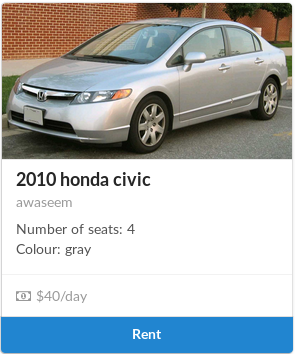
\includegraphics[keepaspectratio, scale=0.5]{carcard}
    \caption{An example car listing}
    \label{fig:carcard}
\end{figure}

\subsection{Vehicle Information}
To view the vehicle information page for a certain vehicle, click the vehicle's title in its lising on the home page. For example, the title of the vehicle listing in Figure \ref{fig:carcard} is "2010 honda civic".

This will bring you to a page outlining detailed information about the vehicle. A picture is displayed, along with the price, owner, number of seats, color, and a summary. Below this information is a list of comments that users have submitted about the vehicle.

Each vehicle has an information page like this.

\subsection{User Information}
To view the user information page for a certain user, click the username of the vehicle's owner in its listing on the home page or on the Vehicle Information page. For example, the owner of the vehicle in the listing in Figure \ref{fig:carcard} is "awaseem".

This will bring you to a page outlining detailed ifnormation about a perticular user. The user's picture is displayed, along with their name, username, email, and a summary. A listing of all the vehicles they have available for rent are listed to the right of this information. Below this information is a list of comments that other users have submitted about this perticular user.

Each vehicle has an information page like this.

\subsection{Renting a vehicle}
To rent a vehicle, press the blue Rent button in the car listing on either the Home Page, Vehicle Information page, or User Information page. For example, a blue Rent button can be seen on the bottom of figure \ref{fig:carcard}.

This will bring you to a page with the vehicle's listing at the top.

Below this listing, you can choose a start date and an end date for your rental. Clicking the fields will cause a calendar date picker to pop up, reducing the need for keyboard input. When you change a date, the total rental price will be updated and it can be seen directly below the car listing. You may only rent the vehicle over an interval that is not already booked.

Once you are satisfied with the dates and the price, press the green Rent button on the bottom of the page to submit your request to rent the vehicle. The owner must first approve the rental before you may rent it.

After clicking the green Rent button, you will be brought to your Edit Profile page, and the new rental will be added to the section titled Your renting history.

\section{Conclusion}
The design and functional implementation of Renti is completed. This report outlined the technical requirements, database design, user manual of the application. For the database design the relational model, object orientated model, and sample SQL queries which may be a representation of what our Object Relational Mapping layer would do. The general hierarchical structure and user manual was also provided.

\section{Appendix A: Filler Data}
The following is the filler data that is used to set up the database. It will be automatically added during an `npm install'.
\lstinputlisting[breaklines, style=js]{../../seeds/filler.js}

\end{document}
